\scanpage{215}
(Résulte de la \unsure{conjonction} des conj de Hodge et de Tate
\inserted{\figure{\begin{tikzpicture}[baseline=(n.base)]\node[draw,ellipse] (n) {sous forme faible};\end{tikzpicture}}},
du moins si $X$ \uline{connexe}).
\uline{\uuline{Caractériser \deleted{de} l'image}} ??

\margin{\figure{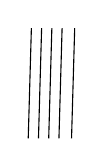
\begin{tikzpicture}\foreach \x in {0,.13,.26,.39,.55}{\draw (\x,0)--(\x+.04,1.4);}\end{tikzpicture}}}

\unsure{M} conclusion si $X$ défini sur $k\subset\mathbf C$, $k$ alg. clos, p.ex. $k=\overline{\mathbf Q}$.

\uline{Analyser l'exemple de Serre de $\pi_1$ non isomorphes}

[\uline{Cas corps de base} $\mathbf R$: tout pt \deleted{\unsure{réel}} \inserted{$a$} définit une $\xi_a\in T_\alpha(\mathbf Z)$.
Tous ces $\xi_a$ sont isomorphes \unsure{pour|puis} si \deleted{\unsure{a}} $X$ est
\deleted{\unsure{géom.} connexe, \unsure{sinon}}
\inserted{\unsure{irrid|irred} (pas néc. géom \unsure{irrid|irred})}
\deleted{il peut y en avoir deux non isom.}
\unsure{Si $a$} est un pt réel, alors $\xi_{\unsure{a|b}}$ \unsure{admet} un autom $\operatorname{frob}_\infty$ d'ordre 2, qui avec la comp. conn. de $G(X,\xi)$ engendre $G(X,\xi)$.

\margin{\diagram{\begin{tikzcd}[column sep=8pt,row sep=9pt]
&X\arrow[dl,no head]\arrow[dd,no head]\\
\mathbf C\arrow[dr,no head]&\\
&\mathbf R
\end{tikzcd}}}

Le foncteur
\[
M\mathrel{\unsure{\mapsto|\sim}}
(\unsure{\xi(M_\xi)|\xi(M)},+\text{structure de Hodge}+\text{involution définie par }\operatorname{frob}_\infty)
\]
est pleinement fidèle.]

\uline{Pb} étudier comment varie la structure de Hodge sur un pt \inserted{complexe} variable,
\uline{en fonction de} la \uline{donnée \unsure{départ}} en le pt $a_0$.

\margin{\figure{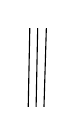
\begin{tikzpicture}\draw (0,0)--(.02,1);\draw (.1,0)--(.12,1);\draw (.2,0)--(.23,1);\end{tikzpicture}}}
\margin{214}
